\documentclass{beamer}
\usepackage[utf8]{inputenc}
\usepackage{graphicx, epsfig}
\usepackage{amsmath,mathrsfs,amsfonts,amssymb}
\usepackage{floatflt}
\usepackage{epic,ecltree}
\usepackage{mathtext}
\usepackage{fancybox}
\usepackage{fancyhdr}
\usepackage{multirow}
\usepackage{enumerate}
\usepackage{epstopdf}
\usepackage{multicol}
\usepackage{algorithm}
\usepackage[noend]{algorithmic}
\usepackage{tikz}
\usepackage{blindtext}
\usetheme{default}%{Singapore}%{Warsaw}%{Warsaw}%{Darmstadt}
\usecolortheme{default}

\setbeamerfont{title}{size=\Huge}
\setbeamertemplate{footline}[page number]{}

\setbeamertemplate{section in toc}[sections numbered]


\makeatletter
\newcommand\HUGE{\@setfontsize\Huge{35}{40}}
\makeatother    

\setbeamerfont{title}{size=\HUGE}
\beamertemplatenavigationsymbolsempty

% latin bold lower
\newcommand{\ba}{\mathbf{a}} 
\newcommand{\bc}{\mathbf{c}} 
\newcommand{\be}{\mathbf{e}} 
\newcommand{\bh}{\mathbf{h}} 
\newcommand{\bp}{\mathbf{p}} 
\newcommand{\bt}{\mathbf{t}} 
\newcommand{\bs}{\mathbf{s}} 
\newcommand{\bu}{\mathbf{u}} 
\newcommand{\bv}{\mathbf{v}} 
\newcommand{\bw}{\mathbf{w}} 
\newcommand{\bx}{\mathbf{x}} 
\newcommand{\by}{\mathbf{y}} 
\newcommand{\bz}{\mathbf{z}} 

% latin bold upper
\newcommand{\bA}{\mathbf{A}} 
\newcommand{\bB}{\mathbf{B}} 
\newcommand{\bC}{\mathbf{C}} 
\newcommand{\bI}{\mathbf{I}} 
\newcommand{\bJ}{\mathbf{J}} 
\newcommand{\bL}{\mathbf{L}} 
\newcommand{\bM}{\mathbf{M}} 
\newcommand{\bP}{\mathbf{P}}
\newcommand{\bQ}{\mathbf{Q}} 
\newcommand{\bR}{\mathbf{R}} 
\newcommand{\bT}{\mathbf{T}} 
\newcommand{\bU}{\mathbf{U}} 
\newcommand{\bV}{\mathbf{V}} 
\newcommand{\bW}{\mathbf{W}} 
\newcommand{\bX}{\mathbf{X}} 
\newcommand{\bY}{\mathbf{Y}} 
\newcommand{\bZ}{\mathbf{Z}} 

% latin cal upper
\newcommand{\cF}{\mathcal{F}} 
\newcommand{\cG}{\mathcal{G}} 
\newcommand{\cI}{\mathcal{I}} 
\newcommand{\cL}{\mathcal{L}} 
\newcommand{\cM}{\mathcal{M}} 
\newcommand{\cN}{\mathcal{N}} 
\newcommand{\cS}{\mathcal{S}} 
\newcommand{\cT}{\mathcal{T}} 
\newcommand{\cW}{\mathcal{W}} 
\newcommand{\cX}{\mathcal{X}} 
\newcommand{\cZ}{\mathcal{Z}} 

% latin bb upper
\newcommand{\bbE}{\mathbb{E}} 
\newcommand{\bbI}{\mathbb{I}} 
\newcommand{\bbP}{\mathbb{P}} 
\newcommand{\bbR}{\mathbb{R}} 

% greek bold lower
\newcommand{\bepsilon}{\boldsymbol{\epsilon}} 
\newcommand{\btheta}{\boldsymbol{\theta}} 
\newcommand{\blambda}{\boldsymbol{\lambda}} 
\newcommand{\bpi}{\boldsymbol{\pi}} 
\newcommand{\bmu}{\boldsymbol{\mu}} 
\newcommand{\bsigma}{\boldsymbol{\sigma}} 
\newcommand{\bphi}{\boldsymbol{\phi}} 

% greek bold upper
\newcommand{\bSigma}{\boldsymbol{\Sigma}} 

\DeclareMathOperator*{\argmin}{arg\,min}
\DeclareMathOperator*{\argmax}{arg\,max}

\newcommand{\createdgmtitle}[1]{\title[\hbox to 56mm{Deep Generative Models  \hfill\insertframenumber\,/\,\inserttotalframenumber}]
	{\vspace{1cm} \\ Deep Generative Models \\ {\Huge Lecture #1}}
	\author{Roman Isachenko}
	\institute{
	Moscow Institute of Physics and Technology
	} 
	\date{2023, Autumn}
}

\usepackage{tikz}
\usetikzlibrary{arrows,shapes,positioning,shadows,trees}

\newcommand\myfootnote[1]{%
  \tikz[remember picture,overlay]
  \draw (current page.south west) +(1in + \oddsidemargin,0.5em)
  node[anchor=south west,inner sep=0pt]{\parbox{\textwidth}{%
      \rlap{\rule{10em}{0.4pt}}\raggedright\scriptsize \textit{#1}}};}

\newcommand\myfootnotewithlink[2]{%
  \tikz[remember picture,overlay]
  \draw (current page.south west) +(1in + \oddsidemargin,0.5em)
  node[anchor=south west,inner sep=0pt]{\parbox{\textwidth}{%
      \rlap{\rule{10em}{0.4pt}}\raggedright\scriptsize\href{#1}{\textit{#2}}}};}
      
\AtBeginSection[]
      {
      	\begin{frame}{Outline}
      		\tableofcontents[currentsection]
      	\end{frame}
      }
      \AtBeginSubsection[]{
      	\begin{frame}{Outline}
      		\tableofcontents[currentsection,currentsubsection]
      	\end{frame}
}
\createdgmtitle{11}

\usepackage{tikz}

\usetikzlibrary{arrows,shapes,positioning,shadows,trees}
%--------------------------------------------------------------------------------
\begin{document}
%--------------------------------------------------------------------------------
\begin{frame}[noframenumbering,plain]
%\thispagestyle{empty}
\titlepage
\end{frame}
%=======
\begin{frame}{Recap of previous lecture}
	Consider Ordinary Differential Equation    
	\begin{align*}
	    \frac{d \bz(t)}{dt} &= f_{\btheta}(\bz(t), t); \quad \text{with initial condition }\bz(t_0) = \bz_0. \\
	    \bz(t_1) &= \int^{t_1}_{t_0} f_{\btheta}(\bz(t), t) d t  + \bz_0 = \text{ODESolve}(\bz(t_0), f_{\btheta}, t_0,t_1).
	\end{align*}
	\vspace{-0.4cm}
	\begin{block}{Euler update step}
		\vspace{-0.6cm}
		\[
			\frac{\bz(t + \Delta t) - \bz(t)}{\Delta t} = f_{\btheta}(\bz(t), t) \,\, \Rightarrow \,\, \bz(t + \Delta t) = \bz(t) + \Delta t \cdot f_{\btheta}(\bz(t), t)
		\]
		\vspace{-0.7cm}
	\end{block}
	\begin{block}{Residual block}
		\vspace{-0.4cm}
		\[
			\bz_{t + 1} = \bz_t + f_{\btheta}(\bz_t)
		\]
		It is equivalent to Euler update step for solving ODE with $\Delta t = 1$!
	\end{block}
	In the limit of adding more layers and taking smaller steps we get: 
	\[
	    \frac{d \bz(t)}{dt} = f_{\btheta}(\bz(t), t); \quad \bz(t_0) = \bx; \quad \bz(t_1) = \by.
	\]

	\myfootnotewithlink{https://arxiv.org/abs/1806.07366}{Chen R. T. Q. et al. Neural Ordinary Differential Equations, 2018}   
\end{frame}
%=======
\begin{frame}{Recap of previous lecture}
	\begin{block}{Forward pass (loss function)}
		\vspace{-0.8cm}
		\begin{align*}
			L(\by) = L(\bz(t_1)) &= L\left( \bz(t_0) + \int_{t_0}^{t_1} f_{\btheta}(\bz(t), t) dt \right) \\ &= L\bigl(\text{ODESolve}(\bz(t_0), f_{\btheta}, t_0,t_1) \bigr)
		\end{align*}
	\vspace{-0.5cm}
	\end{block}
	\textbf{Note:} ODESolve could be any method (Euler step, Runge-Kutta methods).
	\begin{block}{Backward pass (gradients computation)}
		For fitting parameters we need gradients:
		\[
			\ba_{\bz}(t) = \frac{\partial L(\by)}{\partial \bz(t)}; \quad \ba_{\btheta}(t) = \frac{\partial L(\by)}{\partial \btheta(t)}.
		\]
		In theory of optimal control these functions called \textbf{adjoint} functions. 
		They show how the gradient of the loss depends on the hidden state~$\bz(t)$ and parameters $\btheta$.
	\end{block}

	\myfootnotewithlink{https://arxiv.org/abs/1806.07366}{Chen R. T. Q. et al. Neural Ordinary Differential Equations, 2018}     
\end{frame}
%=======
\begin{frame}{Recap of previous lecture}
		\vspace{-0.3cm}
		\[
		\ba_{\bz}(t) = \frac{\partial L(\by)}{\partial \bz(t)}; \quad \ba_{\btheta}(t) = \frac{\partial L(\by)}{\partial \btheta(t)} \text{-- adjoint functions}.
		\]
		\vspace{-0.3cm}
	\begin{block}{Theorem (Pontryagin)}
	\vspace{-0.6cm}
	\[
		\frac{d \ba_{\bz}(t)}{dt} = - \ba_{\bz}(t)^T \cdot \frac{\partial f_{\btheta}(\bz(t), t)}{\partial \bz}; \quad \frac{d \ba_{\btheta}(t)}{dt} = - \ba_{\bz}(t)^T \cdot \frac{\partial f_{\btheta}(\bz(t), t)}{\partial \btheta}.
	\]
	\vspace{-0.6cm}
	\end{block}
	\begin{block}{Forward pass}
		\vspace{-0.5cm}
		\[
		\bz(t_1) = \int^{t_1}_{t_0} f_{\btheta}(\bz(t), t) d t  + \bz_0 \quad \Rightarrow \quad \text{ODE Solver}
		\]
		\vspace{-0.6cm}
	\end{block}
	\begin{block}{Backward pass}
		\vspace{-0.6cm}
		\begin{equation*}
			\left.
			{\footnotesize 
				\begin{aligned}
					\frac{\partial L}{\partial \btheta(t_0)} &= \ba_{\btheta}(t_0) =  - \int_{t_1}^{t_0} \ba_{\bz}(t)^T \frac{\partial f_{\btheta}(\bz(t), t)}{\partial \btheta(t)} dt + 0 \\
					\frac{\partial L}{\partial \bz(t_0)} &= \ba_{\bz}(t_0) =  - \int_{t_1}^{t_0} \ba_{\bz}(t)^T \frac{\partial f_{\btheta}(\bz(t), t)}{\partial \bz(t)} dt + \frac{\partial L}{\partial \bz(t_1)} \\
					\bz(t_0) &= - \int^{t_0}_{t_1} f_{\btheta}(\bz(t), t) d t  + \bz_1.
				\end{aligned}
			}
			\right\rbrace
			\Rightarrow
			\text{ODE Solver}
		\end{equation*}
		\vspace{-0.4cm} 
	\end{block}
	\myfootnotewithlink{https://arxiv.org/abs/1806.07366}{Chen R. T. Q. et al. Neural Ordinary Differential Equations, 2018}   
\end{frame}
%=======
\begin{frame}{Recap of previous lecture}
	\begin{block}{Continuous-in-time normalizing flows}
		\vspace{-0.5cm}
		\[
			\frac{d\bz(t)}{dt} = f_{\btheta}(\bz(t), t); \quad \frac{d \log p(\bz(t), t)}{d t} = - \text{tr} \left( \frac{\partial f_{\btheta}(\bz(t), t)}{\partial \bz(t)} \right).
		\]
		\vspace{-0.7cm}
	\end{block}
	\begin{block}{Theorem (Picard)}
		If $f$ is uniformly Lipschitz continuous in $\bz$ and continuous in $t$, then the ODE has a \textbf{unique} solution.
	\end{block}
	\begin{block}{Forward transform + log-density}
		\vspace{-0.4cm}
		\[
			\begin{bmatrix}
				\bx \\
				\log p(\bx | \btheta)
			\end{bmatrix}
			= 
			\begin{bmatrix}
				\bz \\
				\log p(\bz)
			\end{bmatrix} + 
			\int_{t_0}^{t_1} 
			\begin{bmatrix}
				f_{\btheta}(\bz(t), t) \\
				- \text{tr} \left( \frac{\partial f_{\btheta}(\bz(t), t)}{\partial \bz(t)} \right) 
			\end{bmatrix} dt.
		\]
		\vspace{-0.4cm}
	\end{block}	
	\begin{block}{Hutchinson's trace estimator}
		\vspace{-0.3cm}
		\[
		   \log p(\bz(t_1)) = \log p(\bz(t_0)) - \mathbb{E}_{p(\bepsilon)} \int_{t_0}^{t_1} \left[ {\color{violet}\bepsilon^T \frac{\partial f}{\partial \bz}} \bepsilon \right] dt.
		\]
	\end{block}
	\myfootnotewithlink{https://arxiv.org/abs/1810.01367}{Grathwohl W. et al. FFJORD: Free-form Continuous Dynamics for Scalable Reversible Generative Models, 2018} 
\end{frame}
%=======
\begin{frame}{Recap of previous lecture}
	\vspace{-0.2cm}
	\begin{block}{SDE basics}
		Let define stochastic process $\bx(t)$ with initial condition $\bx(0) \sim p_0(\bx)$:
		\[
			d\bx = \mathbf{f}(\bx, t) dt + g(t) d \bw, 
		\]
		where $\bw(t)$ is the standard Wiener process (Brownian motion)
		\vspace{-0.2cm}
		\[		
			\bw(t) - \bw(s) \sim \cN(0, (t - s) \bI), \quad d \bw = \bepsilon \cdot \sqrt{dt}, \, \text{where } \bepsilon \sim \cN(0, \bI).
		\]
	\end{block}
	\vspace{-0.5cm}
	\begin{block}{Langevin dynamics}
		Let $\bx_0$ be a random vector. Then under mild regularity conditions for small enough $\eta$ samples from the following dynamics
		\vspace{-0.2cm}
		\[
			\bx_{t + 1} = \bx_t + \eta \frac{1}{2} \nabla_{\bx_t} \log p(\bx_t | \btheta) + \sqrt{\eta} \cdot \bepsilon, \quad \bepsilon \sim \cN(0, \bI).
		\]
		will comes from $p(\bx | \btheta)$.
	\end{block}
	The density $p(\bx | \btheta)$ is a \textbf{stationary} distribution for the Langevin SDE.
	\myfootnotewithlink{https://www.stats.ox.ac.uk/~teh/research/compstats/WelTeh2011a.pdf}{Welling M. Bayesian Learning via Stochastic Gradient Langevin Dynamics, 2011}
\end{frame}
%=======
\begin{frame}{Outline}
	\tableofcontents
\end{frame}
%=======
\section{Score matching}
%=======
\begin{frame}{Generative models zoo}
	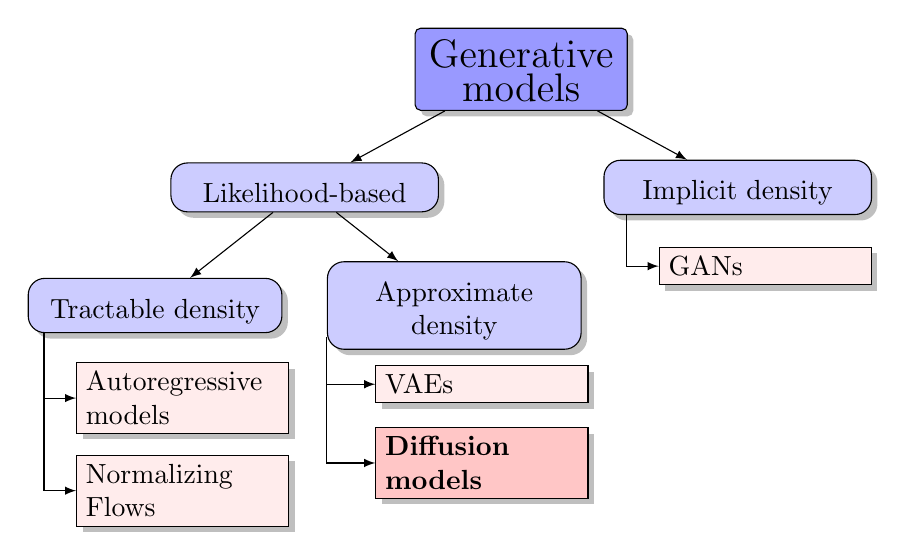
\begin{tikzpicture}[
		basic/.style  = {draw, text width=2cm, drop shadow, rectangle},
		root/.style   = {basic, rounded corners=2pt, thin, text height=1.1em, text width=7em, align=center, fill=blue!40},
		level 1/.style={sibling distance=55mm},
		level 2/.style = {basic, rounded corners=6pt, thin, align=center, fill=blue!20, text height=1.1em, text width=9em, sibling distance=38mm},
		level 3/.style = {basic, rounded corners=6pt, thin,align=center, fill=blue!20, text width=8.5em},
		level 4/.style = {basic, thin, align=left, fill=pink!30, text width=7em},
		level 5/.style = {basic, thin, align=left, fill=pink!90, text width=7em},
		edge from parent/.style={->,draw},
		>=latex]
		
		% root of the the initial tree, level 1
		\node[root] {\Large Generative models}
		% The first level, as children of the initial tree
		child {node[level 2] (c1) {Likelihood-based}
			child {node[level 3] (c11) {Tractable density}}
			child {node[level 3] (c12) {Approximate density}}
		}
		child {node[level 2] (c2) {Implicit density}};
		
		% The second level, relatively positioned nodes
		\begin{scope}[every node/.style={level 4}]
			\node [below of = c11, yshift=-5pt, xshift=10pt] (c111) {Autoregressive models};
			\node [below of = c111, yshift=-5pt] (c112) {Normalizing Flows};
			\node [below of = c12, xshift=10pt] (c121) {VAEs};
			
			\node [below of = c2, xshift=10pt] (c21) {GANs};
		\end{scope}
		
		% The second level, relatively positioned nodes
		\begin{scope}[every node/.style={level 5}]
			\node [below of = c121] (c122) {\textbf{Diffusion \\ models}};
		\end{scope}
		
		% lines from each level 1 node to every one of its "children"
		\foreach \value in {1,2}
		\draw[->] (c11.194) |- (c11\value.west);
		
		\foreach \value in {1,2}
		\draw[->] (c12.194) |- (c12\value.west);
		
		\draw[->] (c2.194) |- (c21.west);
		
	\end{tikzpicture}
\end{frame}
%=======
\begin{frame}{Score matching}
	We could sample from the model using Langevin dynamics if we have $\nabla_{\bx}\log p(\bx| \btheta)$.
	\begin{block}{Fisher divergence}
		\vspace{-0.3cm}
		\[
		D_F(\pi, p) = \frac{1}{2}\bbE_{\pi}\bigl\| \nabla_{\bx}\log p(\bx| \btheta) - \nabla_\bx \log \pi(\bx) \bigr\|^2_2 \rightarrow \min_{\btheta}
		\]
		\vspace{-0.5cm}
	\end{block}
	Let introduce \textbf{score function} $\bs_{\btheta}(\bx) = \nabla_{\bx}\log p(\bx| \btheta)$. 
	\vspace{-0.2cm}
	\begin{figure}
		\centering
		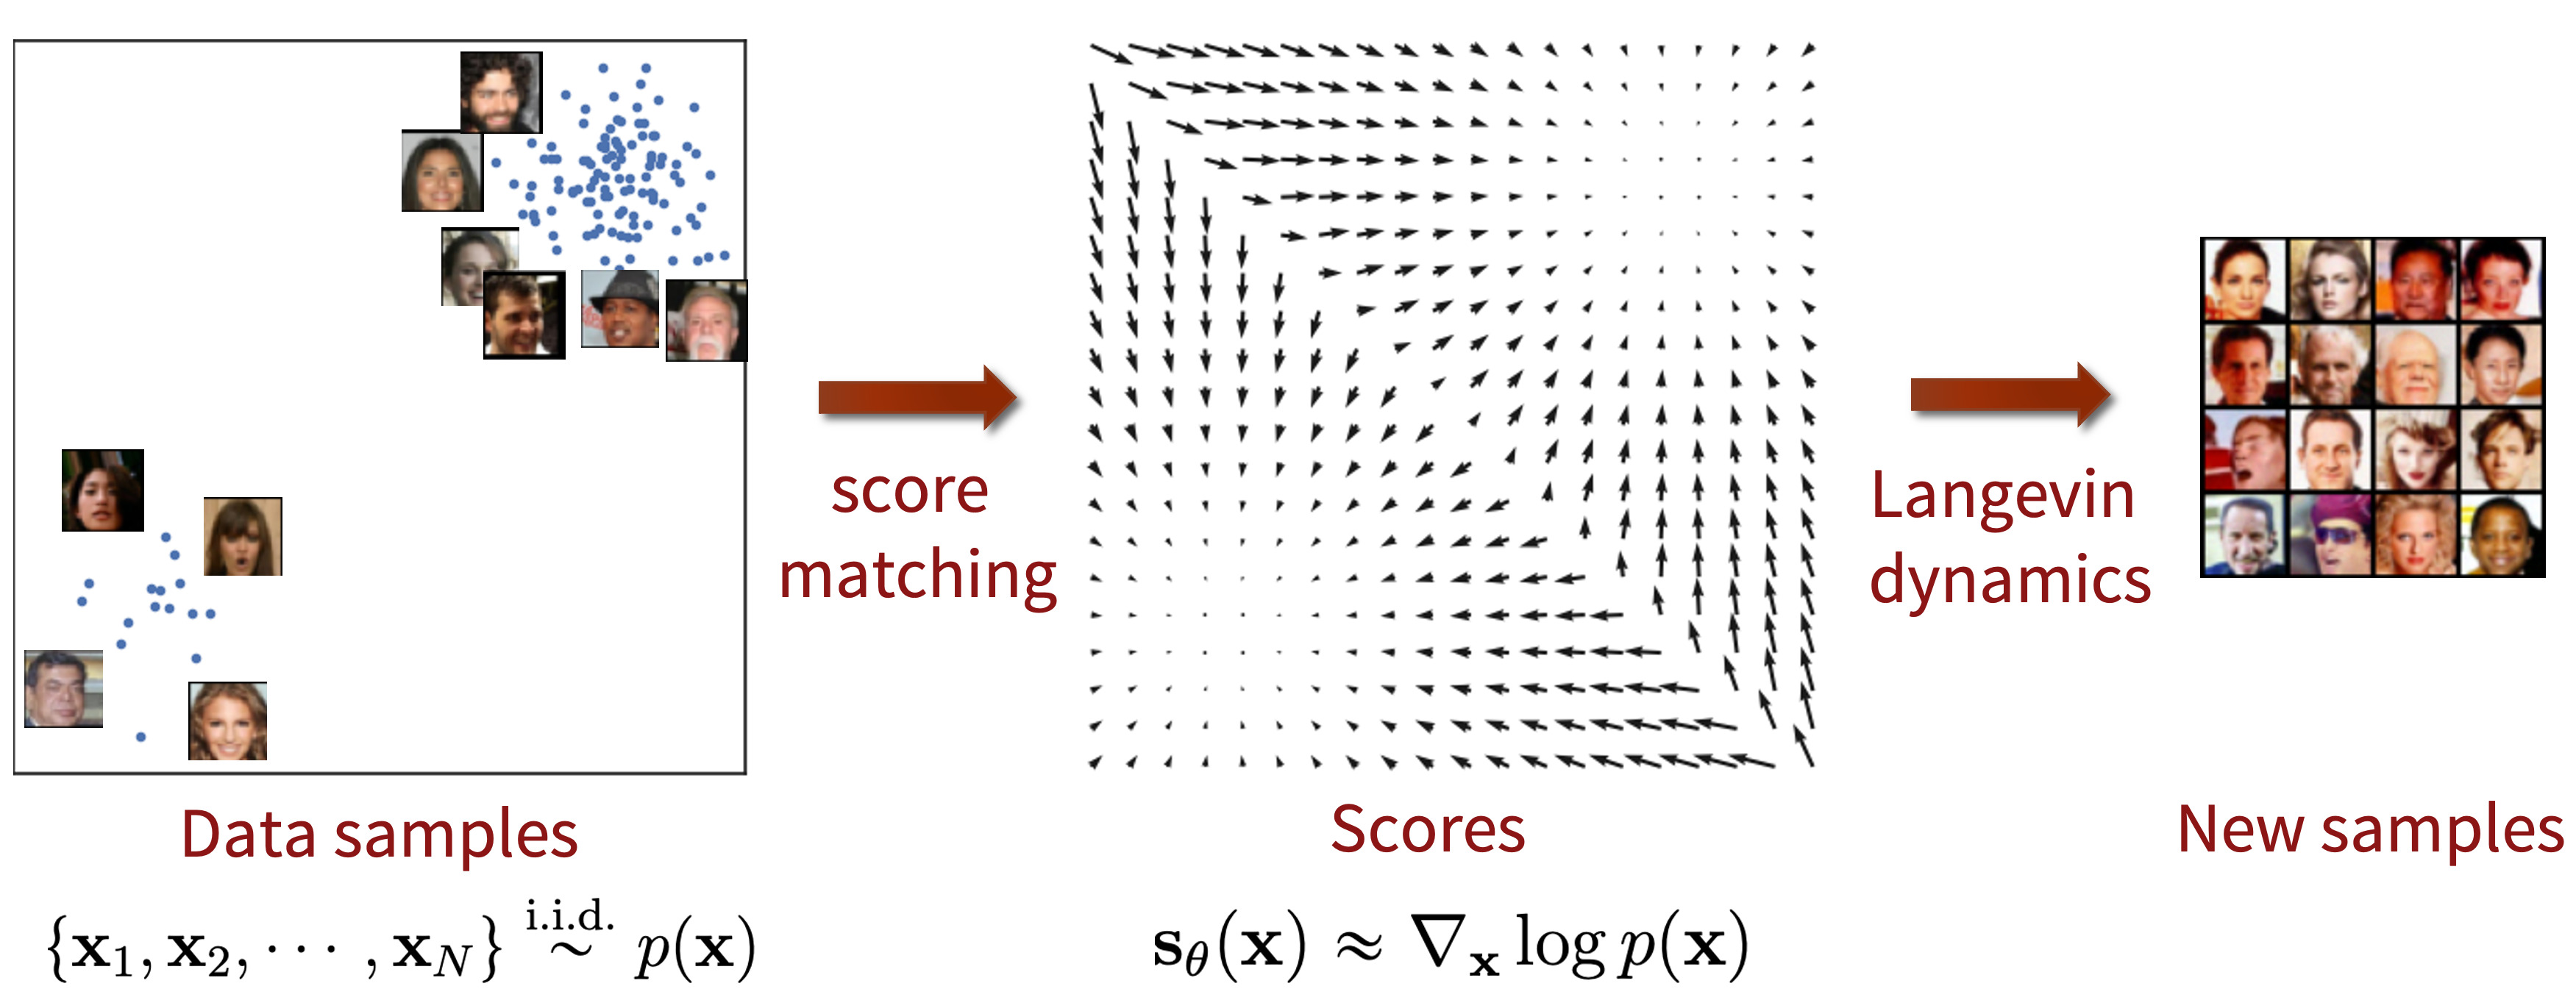
\includegraphics[width=0.75\linewidth]{figs/smld}
	\end{figure}
	\vspace{-0.3cm} 
	\textbf{Problem:} we do not know $\nabla_\bx \log \pi(\bx)$.
	\myfootnotewithlink{https://yang-song.github.io/blog/2021/score/}{Song Y. Generative Modeling by Estimating Gradients of the Data Distribution, blog post, 2021}
\end{frame}
%=======
\begin{frame}{Score matching}
	\begin{block}{Theorem (implicit score matching)}
		Under some regularity conditions, it holds
		\vspace{-0.2cm}
		\[
		\frac{1}{2} \bbE_{\pi}\bigl\| \bs_{\btheta}(\bx) - \nabla_\bx \log \pi(\bx) \bigr\|^2_2 = \bbE_{\pi}\Bigr[ \frac{1}{2}\| \bs_{\btheta}(\bx) \|_2^2 + \text{tr}\bigl(\nabla_{\bx} \bs_{\btheta}(\bx)\bigr) \Bigr] + \text{const}
		\]
		\vspace{-0.6cm}
	\end{block}
	\begin{block}{Proof (only for 1D)}
		\vspace{-0.6cm}
		{\small
			\begin{multline*}
				\bbE_{\pi}\bigl\| s(x) - \nabla_x \log \pi(x) \bigr\|^2_2 = \bbE_{\pi} \bigl[ s(x)^2 + (\nabla_x \log \pi(x))^2 - 2{\color{teal}[s(x) \nabla_x \log \pi(x) ] \bigr] }
			\end{multline*}
			\vspace{-0.8cm}
			\begin{align*}
				{\color{teal}\bbE_{\pi} [{\color{violet}s(x) } \nabla_x \log \pi(x) ] } &= \int {\color{olive}\pi(x) {\color{violet}\nabla_x \log p(x)} \nabla_x \log \pi(x)} d x \\ 
				&= \int {\color{violet}\nabla_x \log p(x) } {\color{olive}\nabla_x \pi(x) } dx = \Bigl.\pi(x) \nabla_x \log p(x) \Bigr|_{-\infty}^{+\infty} \\
				&- \int \nabla^2_x \log p(x)  \pi(x) dx =- \bbE_{\pi} \nabla^2_x \log p(x) =- \bbE_{\pi} \nabla_x s(x)
			\end{align*}
			\[
			\frac{1}{2} \bbE_{\pi}\bigl\| s(x) - \nabla_x \log \pi(x) \bigr\|^2_2 = \bbE_{\pi} \Bigr[\frac{1}{2} s(x)^2 + \nabla_x s(x) \Bigl]+ \text{const}.
			\]
		}
	\end{block}
	\myfootnotewithlink{https://jmlr.org/papers/volume6/hyvarinen05a/old.pdf}{Hyvarinen A. Estimation of non-normalized statistical models by score matching, 2005} 
\end{frame}
%=======
\begin{frame}{Score matching}
	\vspace{-0.3cm}
	\begin{block}{Theorem (implicit score matching)}
		\vspace{-0.6cm}
		\[
		{\color{violet}\frac{1}{2} \bbE_{\pi}\bigl\| \bs_{\btheta}(\bx) - \nabla_\bx \log \pi(\bx) \bigr\|^2_2} = {\color{teal}\bbE_{\pi}\Bigr[ \frac{1}{2}\| \bs_{\btheta}(\bx) \|_2^2 + \text{tr}\bigl(\nabla_{\bx} \bs_{\btheta}(\bx)\bigr) \Bigr]} + \text{const}
		\]
		Here $\nabla_{\bx} \bs_{\btheta}(\bx) = \nabla_{\bx}^2 \log p(\bx | \btheta)$ is a Hessian matrix.
	\end{block}
	\begin{enumerate}
		\item {\color{violet}The left hand side} is intractable due to unknown $\pi(\bx)$ -- \textbf{denoising score matching}. 
		\item {\color{teal}The right hand side} is complex due to Hessian matrix -- \textbf{sliced score matching}.
	\end{enumerate}
	\begin{block}{Sliced score matching (Hutchinson's trace estimation)}
	\vspace{-0.3cm}
	\[
		\text{tr}\bigl(\nabla_{\bx} \bs_{\btheta}(\bx)\bigr) = \mathbb{E}_{p(\bepsilon)} \left[ {\color{olive}\bepsilon^T \nabla_{\bx} \bs_{\btheta}(\bx)} \bepsilon \right]
	\]
	\end{block}
	\myfootnote{\href{https://yang-song.net/blog/2021/ssm/}{Song Y. Sliced Score Matching: A Scalable Approach to Density and Score Estimation, 2019} \\
	\href{https://yang-song.net/blog/2021/score/}{Song Y. Generative Modeling by Estimating Gradients of the Data Distribution, blog post, 2021}}
\end{frame}
%=======
\begin{frame}{Denoising score matching}
	Let perturb original data $\bx \sim \pi(\bx)$ by random normal noise 
	\[
		\bx' = \bx + \sigma \cdot \bepsilon, \quad \bepsilon \sim \cN(0, 1), \quad p(\bx' | \bx, \sigma) = \cN(\bx' | \bx, \sigma^2 \bI)
	\]
	\vspace{-0.4cm}
	\[
		\pi(\bx' | \sigma) = \int \pi(\bx) p(\bx' | \bx, \sigma) d\bx.
	\]
	\vspace{-0.4cm} \\
	Then the solution of 
	\[
		\frac{1}{2} \bbE_{\pi(\bx' | \sigma)}\bigl\| \bs_{\btheta}(\bx', \sigma) - \nabla_{\bx'} \log \pi(\bx' | \sigma) \bigr\|^2_2 \rightarrow \min_{\btheta}
	\]
	\vspace{-0.3cm} \\
	satisfies $\bs_{\btheta}(\bx', \sigma) \approx \bs_{\btheta}(\bx', 0) = \bs_{\btheta}(\bx)$ if $\sigma$ is small enough.
	\myfootnotewithlink{http://www.iro.umontreal.ca/~vincentp/Publications/smdae_techreport.pdf}{Vincent P. A Connection Between Score Matching and Denoising Autoencoders, 2010}
\end{frame}
%=======
\begin{frame}{Denoising score matching}
	\begin{block}{Theorem}
	\vspace{-0.5cm}
	\begin{multline*}
		\bbE_{\pi(\bx' | \sigma)}\bigl\| \bs_{\btheta}(\bx', \sigma) - \nabla_{\bx'} \log \pi(\bx' | \sigma) \bigr\|^2_2 = \\ = \bbE_{\pi(\bx)} \bbE_{p(\bx' | \bx, \sigma)}\bigl\| \bs_{\btheta}(\bx', \sigma) - \nabla_{\bx'} \log p(\bx' | \bx, \sigma) \bigr\|^2_2 + \text{const}(\btheta)
	\end{multline*}
	\vspace{-0.5cm}
	\end{block}
	\begin{block}{Gradient of the noise kernel}
	\vspace{-0.3cm}
	\[
		\nabla_{\bx'} \log p(\bx' | \bx, \sigma) = \nabla_{\bx'} \log \cN(\bx' | \bx, \sigma^2 \bI) = - \frac{\bx' - \bx}{\sigma^2}
	\]
	\vspace{-0.3cm}
	\end{block}
	\begin{itemize}
		\item The RHS does not need to compute $\nabla_{\bx'} \log \pi(\bx' | \sigma)$ and even $\nabla_{\bx'} \log \pi(\bx')$.
		\item $\bs_{\btheta}(\bx', \sigma)$ tries to \textbf{denoise} a corrupted sample $\bx'$.
		\item Score function $\bs_{\btheta}(\bx', \sigma)$ parametrized by $\sigma$. How to make it?
	\end{itemize}
	\myfootnotewithlink{http://www.iro.umontreal.ca/~vincentp/Publications/smdae_techreport.pdf}{Vincent P. A Connection Between Score Matching and Denoising Autoencoders, 2010}
\end{frame}
%=======
\section{Noise conditioned score network}
%=======
\begin{frame}{Denoising score matching}
	\begin{itemize}
		\item If $\sigma$ is \textbf{small}, the score function is not accurate and Langevin dynamics will probably fail to jump between modes.
		\begin{figure}
			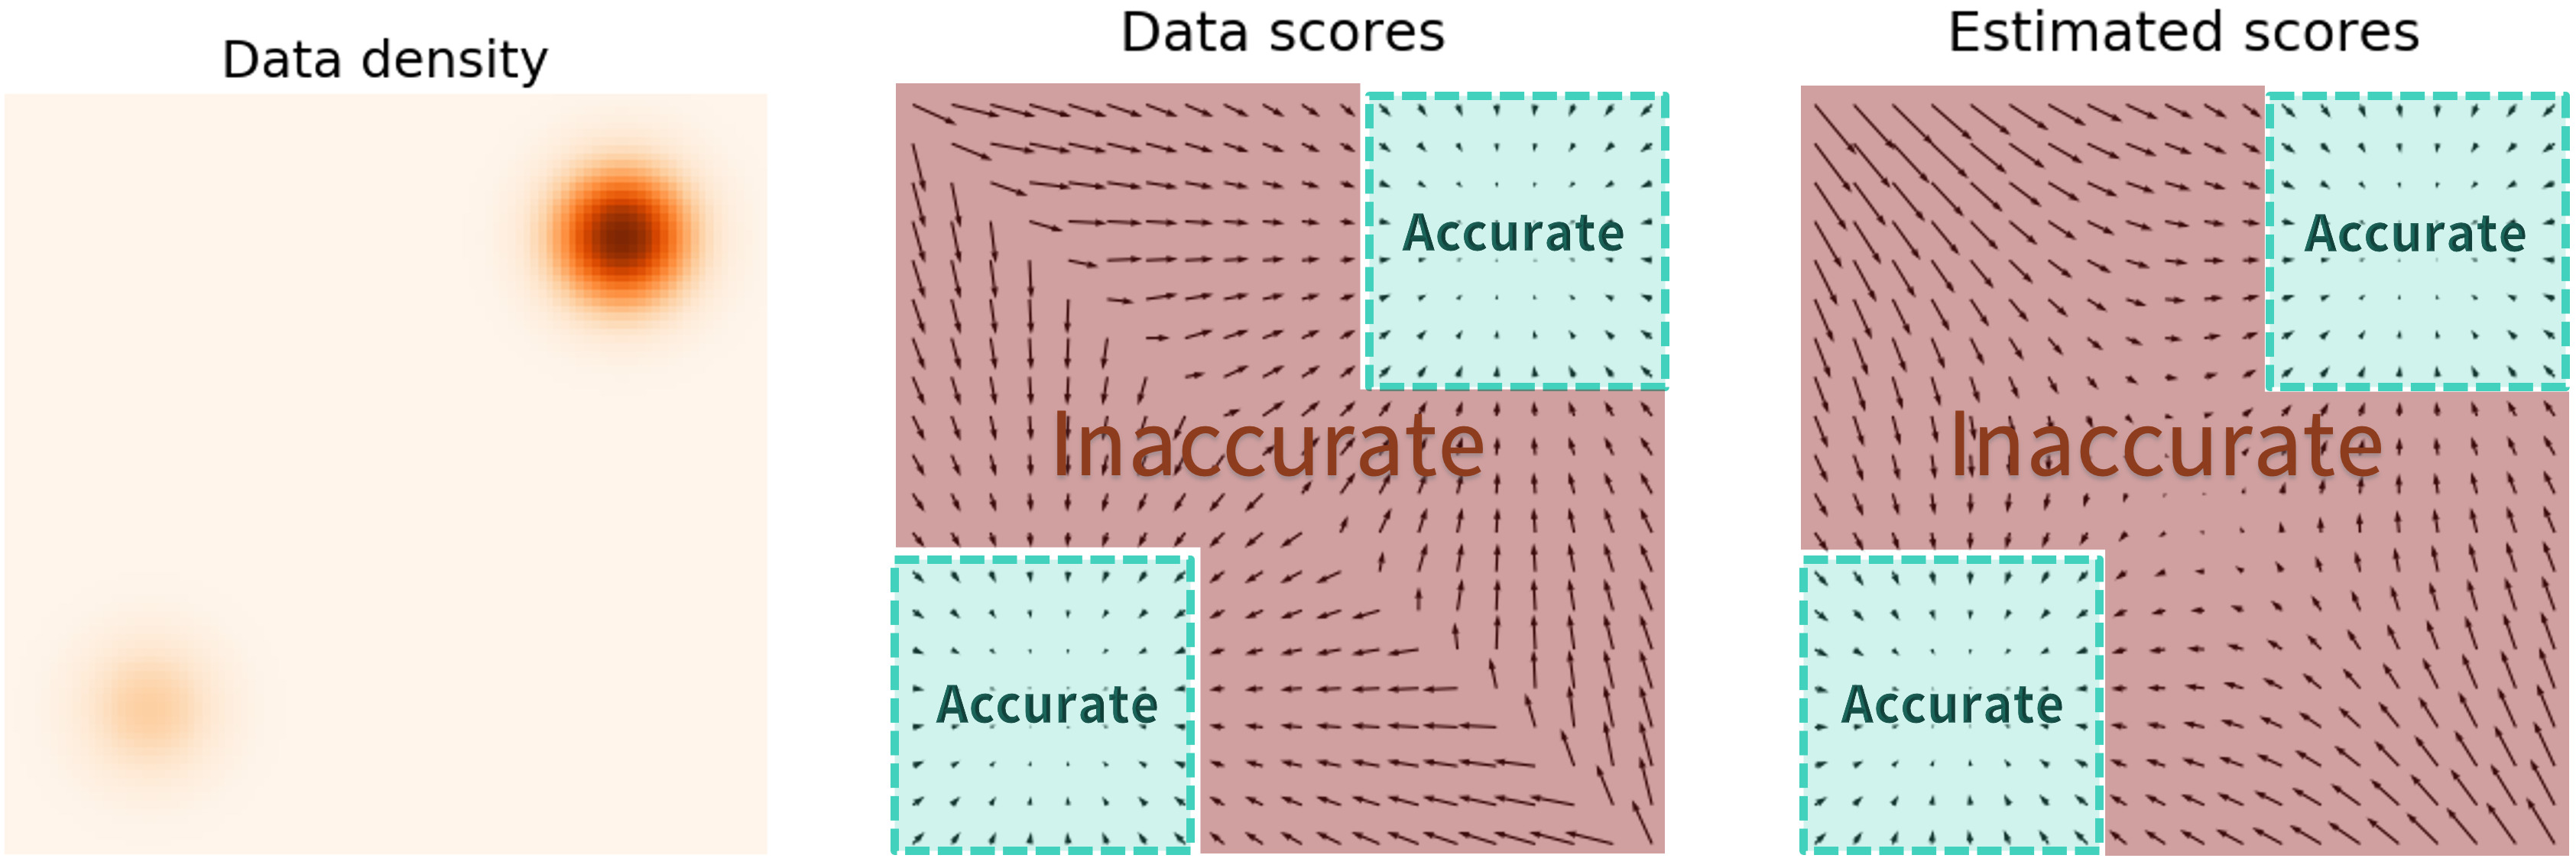
\includegraphics[width=0.75\linewidth]{figs/pitfalls}
		\end{figure}
		\item If $\sigma$ is \textbf{large}, it is good for low-density regions and  multimodal distributions, but we will learn too corrupted distribution.
		\begin{figure}
			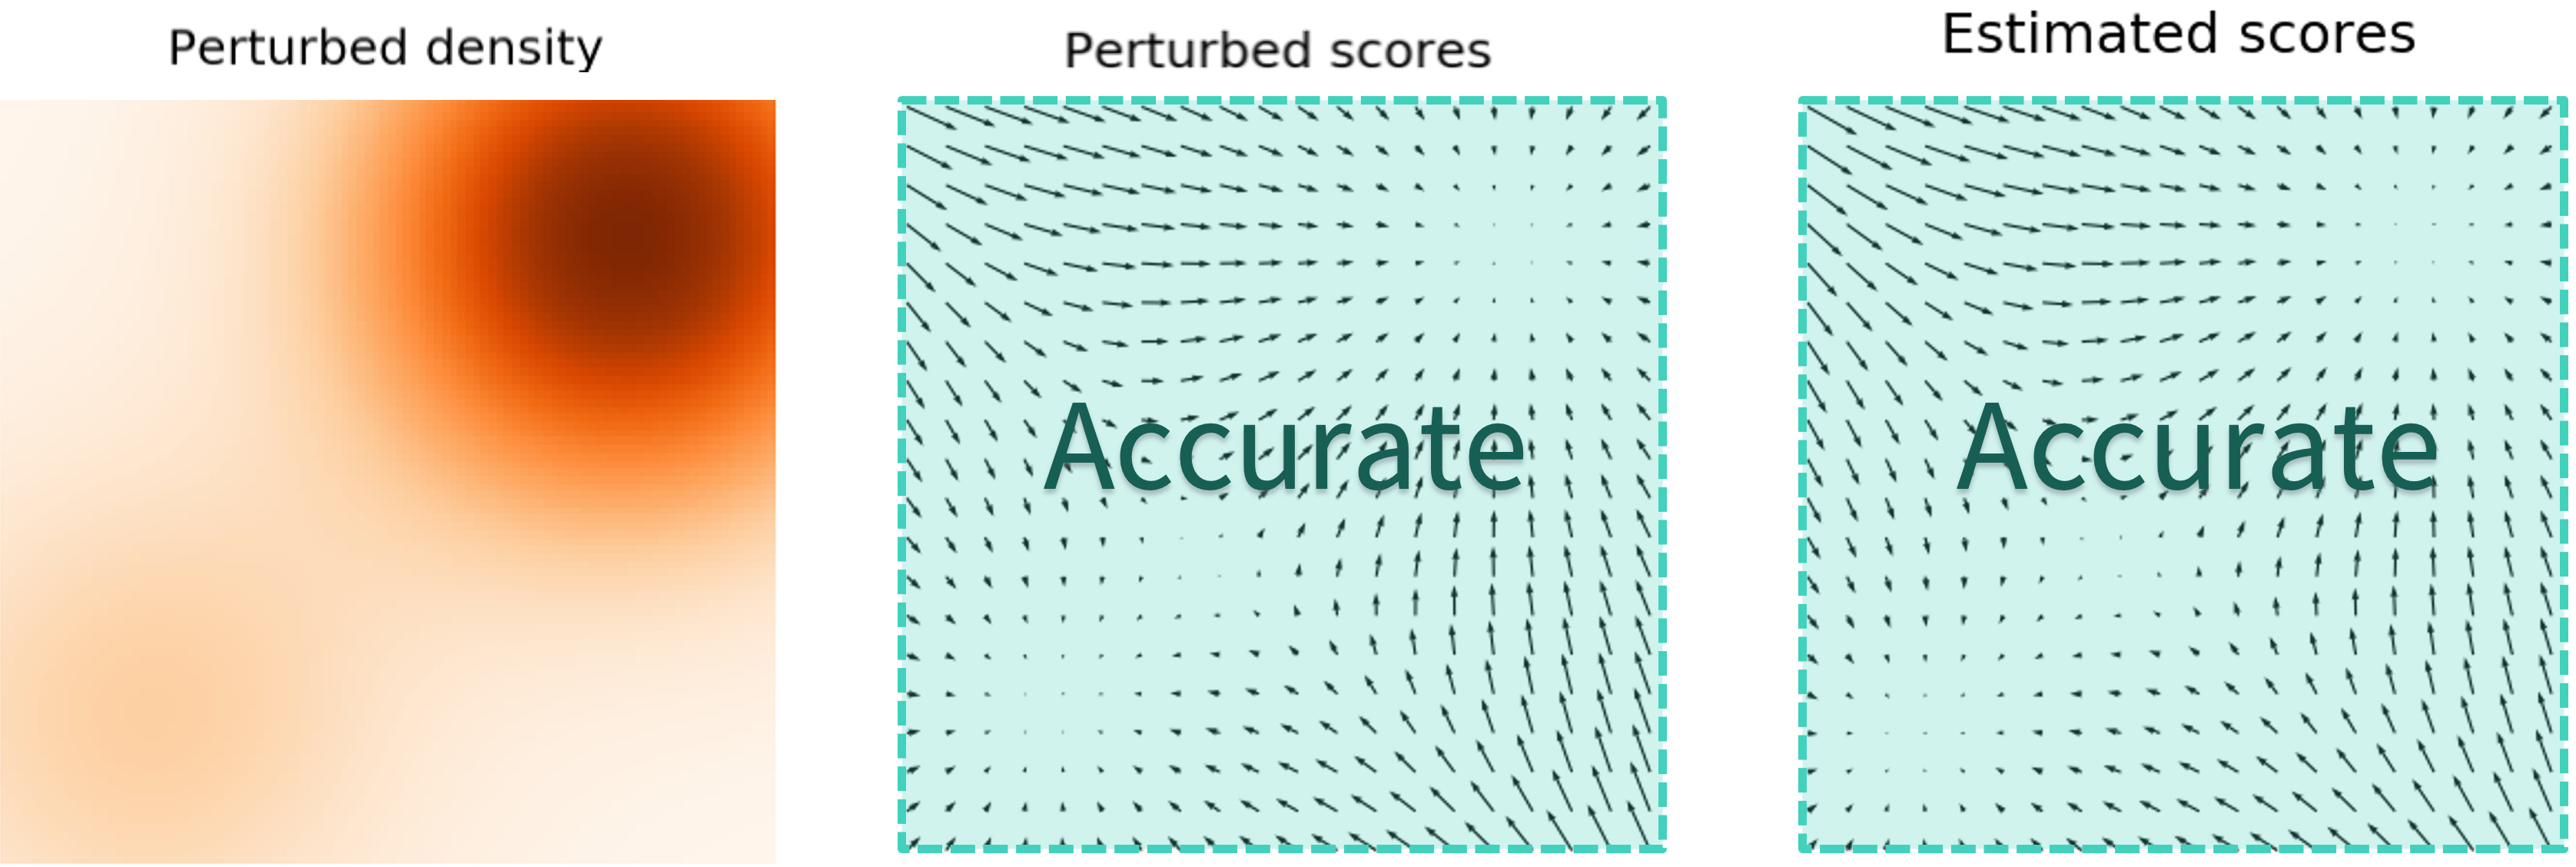
\includegraphics[width=0.75\linewidth]{figs/single_noise}
		\end{figure}
	\end{itemize}
	\myfootnotewithlink{https://yang-song.github.io/blog/2021/score/}{Song Y. Generative Modeling by Estimating Gradients of the Data Distribution, blog post, 2021}
\end{frame}
%=======
\begin{frame}{Noise conditioned score network}
	\begin{itemize}
		\item Define the sequence of noise levels: $\sigma_1 > \sigma_2 > \dots > \sigma_L$.
		\item Perturb the original data with the different noise level to get $\pi(\bx' | \sigma_1), \dots, \pi(\bx' | \sigma_L)$.
		\item Train denoised score function $\bs_{\btheta}(\bx', \sigma)$ for each noise level:
		\vspace{-0.2cm}
		\[
			\sum_{l=1}^L {\color{violet}\sigma_l^2} \bbE_{\pi(\bx)} \bbE_{p(\bx' | \bx, \sigma_l)}\bigl\| \bs_{\btheta}(\bx', \sigma_l) - \nabla_\bx' \log p(\bx' | \bx, \sigma_l) \bigr\|^2_2 \rightarrow \min_{\btheta}
		\]
		\item Sample from \textbf{annealed} Langevin dynamics (for $l=1, \dots, L$).
	\end{itemize}
	\begin{figure}
		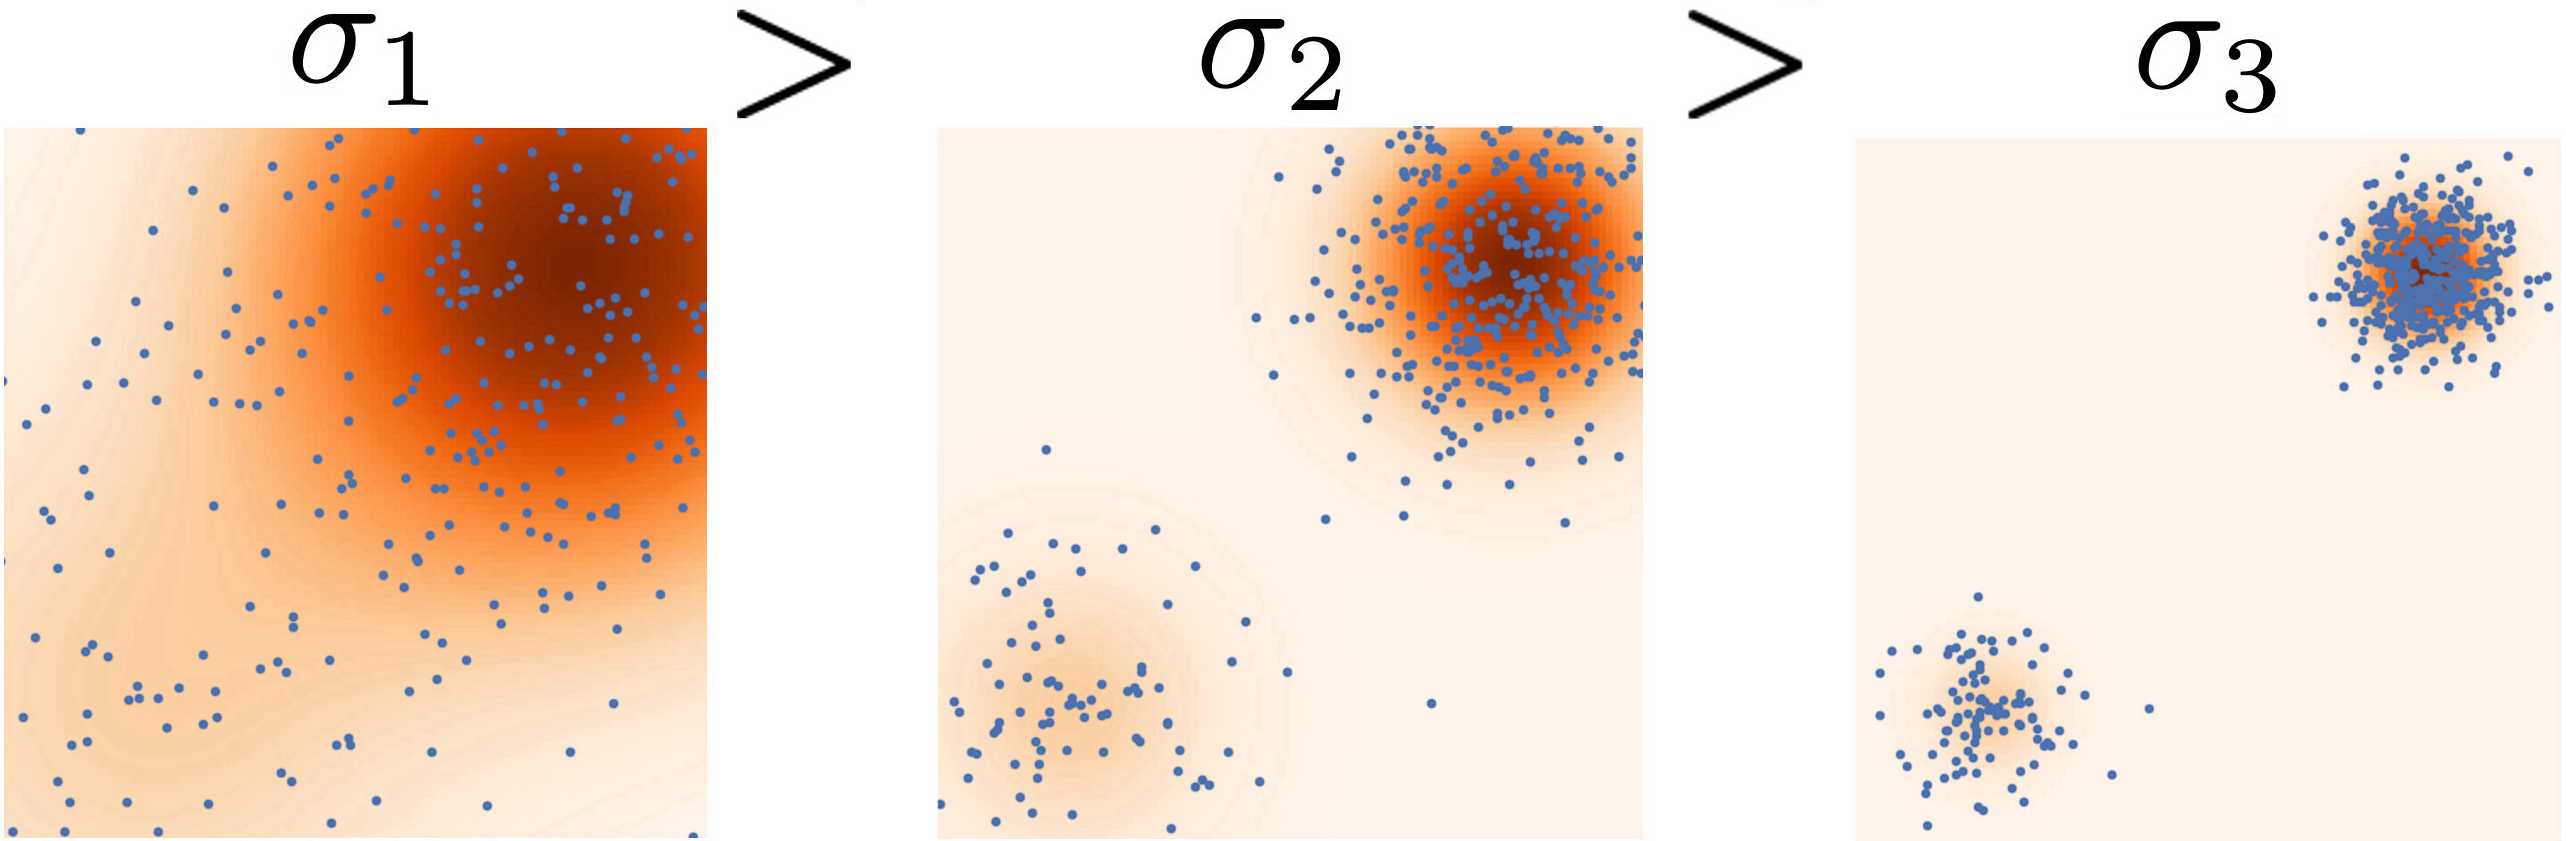
\includegraphics[width=0.6\linewidth]{figs/multi_scale}
	\end{figure}
	\begin{figure}
		
\includegraphics[width=\linewidth]{figs/duoduo}
	\end{figure}
	\myfootnotewithlink{https://arxiv.org/abs/1907.05600}{Song Y. et al. Generative Modeling by Estimating Gradients of the Data Distribution, 2019}
\end{frame}
%=======
\begin{frame}{Noise conditioned score network}
	\begin{minipage}{0.5\linewidth}
		\vspace{-0.7cm}
		\begin{block}{Training: loss function}
			\vspace{-0.8cm}
			\[
			\sum_{i=1}^L \sigma_l^2\bbE_{\pi(\bx)} \bbE_{\bepsilon}\left\| \bs_l + \frac{\bepsilon}{\sigma_l} \right\|^2_2,
			\]
		\end{block}
		\vspace{-0.5cm}
		Here
		\begin{itemize}
			\item $\bs_l = \bs_{\btheta}(\bx + \sigma_l \cdot \bepsilon, \sigma_l)$.
			\item $\nabla_{\bx'} \log p(\bx' | \bx, \sigma) = - \frac{\bx' - \bx}{\sigma^2} = - \frac{\bepsilon}{\sigma_l}$.
		\end{itemize}
	\end{minipage}%
	\begin{minipage}{0.5\linewidth}
		\begin{block}{Inference: annealed Langevin dynamic}
			\begin{figure}
				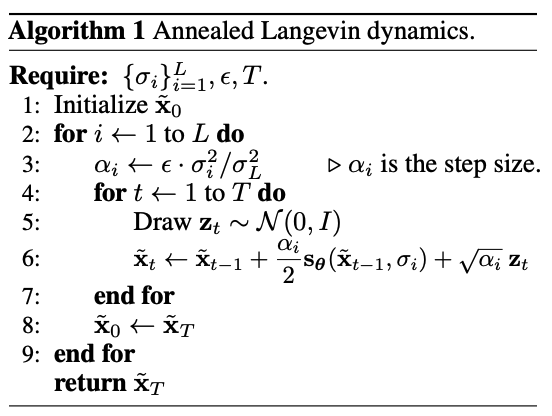
\includegraphics[width=0.9\linewidth]{figs/ald}
			\end{figure}
		\end{block}
	\end{minipage}
	\vspace{-0.7cm}
	\begin{block}{Samples}
		\begin{figure}
			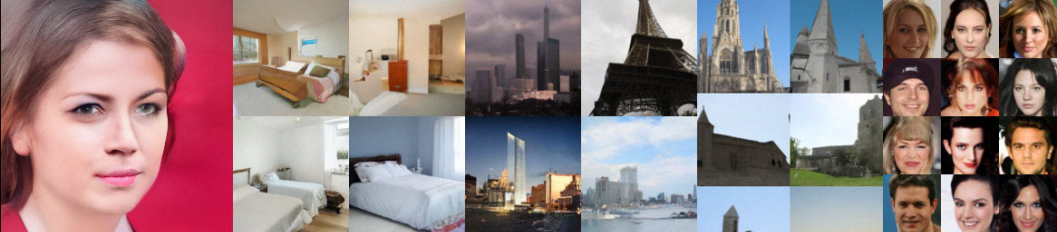
\includegraphics[width=\linewidth]{figs/NCSNv2}
		\end{figure}
	\end{block}
	\myfootnotewithlink{https://arxiv.org/abs/2006.09011}{Song Y. et al. Improved Techniques for Training Score-Based Generative Models, 2020}
\end{frame}
%=======
\begin{frame}{Summary}
	\begin{itemize}
		\item Score matching proposes to minimize Fisher divergence to get score function.
		\vfill
		\item Sliced score matching and denoising score matching are two techniques to get scalable algorithm for fitting Fisher divergence.
		\vfill
		\item Noise conditioned score network uses multiple noise levels and annealed Langevin dynamics to fit score function.
	\end{itemize}
\end{frame}
\end{document} 